% Options for packages loaded elsewhere
\PassOptionsToPackage{unicode}{hyperref}
\PassOptionsToPackage{hyphens}{url}
%
\documentclass[
  a4paper,
]{article}
\usepackage{amsmath,amssymb}
\usepackage{iftex}
\ifPDFTeX
  \usepackage[T1]{fontenc}
  \usepackage[utf8]{inputenc}
  \usepackage{textcomp} % provide euro and other symbols
\else % if luatex or xetex
  \usepackage{unicode-math} % this also loads fontspec
  \defaultfontfeatures{Scale=MatchLowercase}
  \defaultfontfeatures[\rmfamily]{Ligatures=TeX,Scale=1}
\fi
\usepackage{lmodern}
\ifPDFTeX\else
  % xetex/luatex font selection
    \setmainfont[]{Helvetica}
\fi
% Use upquote if available, for straight quotes in verbatim environments
\IfFileExists{upquote.sty}{\usepackage{upquote}}{}
\IfFileExists{microtype.sty}{% use microtype if available
  \usepackage[]{microtype}
  \UseMicrotypeSet[protrusion]{basicmath} % disable protrusion for tt fonts
}{}
\makeatletter
\@ifundefined{KOMAClassName}{% if non-KOMA class
  \IfFileExists{parskip.sty}{%
    \usepackage{parskip}
  }{% else
    \setlength{\parindent}{0pt}
    \setlength{\parskip}{6pt plus 2pt minus 1pt}}
}{% if KOMA class
  \KOMAoptions{parskip=half}}
\makeatother
\usepackage{xcolor}
\usepackage[margin=0.75in]{geometry}
\usepackage{graphicx}
\makeatletter
\newsavebox\pandoc@box
\newcommand*\pandocbounded[1]{% scales image to fit in text height/width
  \sbox\pandoc@box{#1}%
  \Gscale@div\@tempa{\textheight}{\dimexpr\ht\pandoc@box+\dp\pandoc@box\relax}%
  \Gscale@div\@tempb{\linewidth}{\wd\pandoc@box}%
  \ifdim\@tempb\p@<\@tempa\p@\let\@tempa\@tempb\fi% select the smaller of both
  \ifdim\@tempa\p@<\p@\scalebox{\@tempa}{\usebox\pandoc@box}%
  \else\usebox{\pandoc@box}%
  \fi%
}
% Set default figure placement to htbp
\def\fps@figure{htbp}
\makeatother
\setlength{\emergencystretch}{3em} % prevent overfull lines
\providecommand{\tightlist}{%
  \setlength{\itemsep}{0pt}\setlength{\parskip}{0pt}}
\setcounter{secnumdepth}{-\maxdimen} % remove section numbering
\usepackage{titling}
\pretitle{\begin{flushleft}}
\posttitle{\end{flushleft}}
\usepackage{booktabs}
\usepackage{longtable}
\usepackage{float}
\floatplacement{figure}{H}
\usepackage{colortbl}
\usepackage{pdflscape}
\usepackage{tabu}
\usepackage{makecell}
\usepackage{xcolor}
\usepackage{soul}
\usepackage{caption}
\usepackage[singlelinecheck=false]{caption}
\usepackage[font={small,bf}]{caption}
\usepackage{multirow}
\usepackage{array}
\usepackage{lscape}
\newcommand{\blandscape}{\begin{landscape}}
\newcommand{\elandscape}{\end{landscape}}
\usepackage[dvipsnames]{xcolor}
\renewcommand{\footnotesize}{\tiny}
\usepackage{threeparttable}
\usepackage{booktabs}
\usepackage{longtable}
\usepackage{array}
\usepackage{multirow}
\usepackage{wrapfig}
\usepackage{float}
\usepackage{colortbl}
\usepackage{pdflscape}
\usepackage{tabu}
\usepackage{threeparttable}
\usepackage{threeparttablex}
\usepackage[normalem]{ulem}
\usepackage{makecell}
\usepackage{xcolor}
\usepackage{bookmark}
\IfFileExists{xurl.sty}{\usepackage{xurl}}{} % add URL line breaks if available
\urlstyle{same}
\hypersetup{
  hidelinks,
  pdfcreator={LaTeX via pandoc}}

\title{\vspace{-1.5cm} \begin{LARGE} WGS Quality Control Report \end{LARGE}}
\author{}
\date{\vspace{-2.5em}}

\begin{document}
\maketitle

\normalsize Batch Name: 2025-06-20\_A

\normalsize Experiment Name: 25ARS\_KPNGHRU\_LY9BV

\fontsize{7}{8}
\selectfont
\captionsetup[table]{labelformat=empty}
\renewcommand{\arraystretch}{1.2}

\begin{longtable}[t]{>{\centering\arraybackslash}p{1cm}>{\centering\arraybackslash}p{2.8cm}>{\centering\arraybackslash}p{1.5cm}>{\centering\arraybackslash}p{5cm}>{\centering\arraybackslash}p{5cm}}
\toprule
\multicolumn{1}{>{\centering\arraybackslash}p{1cm}}{\cellcolor[HTML]{D4D4D4}{\textbf{Isolate No.}}} & \multicolumn{1}{>{\centering\arraybackslash}p{2.8cm}}{\cellcolor[HTML]{D4D4D4}{\textbf{Sample ID}}} & \multicolumn{1}{>{\centering\arraybackslash}p{1.5cm}}{\cellcolor[HTML]{D4D4D4}{\textbf{Description}}} & \multicolumn{1}{>{\centering\arraybackslash}p{5cm}}{\cellcolor[HTML]{D4D4D4}{\textbf{ARSRL}}} & \multicolumn{1}{>{\centering\arraybackslash}p{5cm}}{\cellcolor[HTML]{D4D4D4}{\textbf{WGS}}}\\
\midrule
1 & 24ARS\_BRH0191 & UDI145 & \em{Klebsiella pneumoniae} & \em{Klebsiella pneumoniae}\\
2 & 24ARS\_BRH0195 & UDI130 & \em{Klebsiella pneumoniae} & \em{Klebsiella pneumoniae}\\
3 & 24ARS\_CRH0210 & UDI128 & \em{Klebsiella pneumoniae} & \em{Klebsiella pneumoniae}\\
4 & 24ARS\_DMC0490 & UDI147 & \em{Klebsiella pneumoniae} & \em{Klebsiella pneumoniae}\\
5 & 24ARS\_BRH0192 & UDI146 & \em{Klebsiella pneumoniae} & \em{Klebsiella pneumoniae}\\
\addlinespace
6 & 24ARS\_DMC0494 & UDI150 & \em{Klebsiella pneumoniae} & \em{Klebsiella pneumoniae}\\
7 & 24ARS\_GMH0269 & UDI151 & \em{Klebsiella pneumoniae} & \em{Klebsiella pneumoniae}\\
8 & 24ARS\_GMH0281 & UDI127 & \em{Klebsiella pneumoniae} & \em{Klebsiella pneumoniae}\\
9 & 24ARS\_DMC0492 & UDI148 & \em{Klebsiella pneumoniae} & \em{Klebsiella pneumoniae}\\
10 & 24ARS\_JLM0248 & UDI153 & \em{Klebsiella pneumoniae} & \em{Klebsiella pneumoniae}\\
\addlinespace
11 & 24ARS\_MAR0317 & UDI132 & \em{Klebsiella pneumoniae} & \em{Klebsiella pneumoniae}\\
12 & 24ARS\_NKI0075 & UDI155 & \em{Klebsiella pneumoniae} & \em{Klebsiella pneumoniae}\\
13 & 24ARS\_JLM0247 & UDI152 & \em{Klebsiella pneumoniae} & \em{Klebsiella pneumoniae}\\
14 & 24ARS\_VSM0556 & UDI161 & \em{Klebsiella pneumoniae} & \em{Klebsiella pneumoniae}\\
15 & 24ARS\_VSM0557 & UDI162 & \em{Klebsiella pneumoniae} & \em{Klebsiella pneumoniae}\\
\addlinespace
16 & 24ARS\_VSM0586 & UDI123 & \em{Klebsiella pneumoniae} & \em{Klebsiella pneumoniae}\\
17 & 24ARS\_VSM0660 & UDI137 & \em{Klebsiella pneumoniae} & \em{Klebsiella pneumoniae}\\
18 & 24ARS\_VSM0662 & UDI139 & \em{Klebsiella pneumoniae} & \em{Klebsiella pneumoniae}\\
19 & 25ARS\_DMC0010 & UDI135 & \em{Klebsiella pneumoniae} & \em{Klebsiella pneumoniae}\\
20 & 25ARS\_GMH0007 & UDI144 & \em{Klebsiella pneumoniae} & \em{Klebsiella pneumoniae}\\
\addlinespace
21 & 25ARS\_MAR0014 & UDI142 & \em{Klebsiella pneumoniae} & \em{Klebsiella pneumoniae}\\
22 & 24ARS\_NKI0077 & UDI157 & \em{Klebsiella pneumoniae} & \em{Klebsiella quasipneumoniae}\\
\bottomrule
\multicolumn{5}{l}{\rule{0pt}{1em}\textit{Legend:} PASS   |   \colorbox{Salmon}{FAILURE}   |   \textcolor{Blue}{EXCEEDS THRESHOLD METRIC/S}   |   (x) - NON-CONCORDANT   |}\\
\end{longtable}

\fontsize{7}{8}
\selectfont
\captionsetup[table]{labelformat=empty}
\renewcommand{\arraystretch}{1.2}

\(\\\) \newpage

\begin{landscape}
\fontsize{7}{8}
\selectfont
\captionsetup[table]{labelformat=empty}
\renewcommand{\arraystretch}{1.2}

\begin{table}[!h]
\centering
\resizebox{\ifdim\width>\linewidth\linewidth\else\width\fi}{!}{
\begin{tabular}{cc>{}ccccccccc}
\toprule
\cellcolor[HTML]{D4D4D4}{\textbf{Isolate No.}} & \cellcolor[HTML]{D4D4D4}{\textbf{Sample ID}} & \cellcolor[HTML]{D4D4D4}{\textbf{WGS ID}} & \cellcolor[HTML]{D4D4D4}{\textbf{completeness}} & \cellcolor[HTML]{D4D4D4}{\textbf{contamination}} & \cellcolor[HTML]{D4D4D4}{\textbf{Depth of coverage}} & \cellcolor[HTML]{D4D4D4}{\textbf{Genome size}} & \cellcolor[HTML]{D4D4D4}{\textbf{GC content}} & \cellcolor[HTML]{D4D4D4}{\textbf{Contig count}} & \cellcolor[HTML]{D4D4D4}{\textbf{N50}} & \cellcolor[HTML]{D4D4D4}{\textbf{Mean read Q-score}}\\
\midrule
1 & 24ARS\_BRH0191 & \em{Klebsiella pneumoniae} & 100 & 0.24 & 72.5 & 5.60 Mb & 57 & 55 & 242827 & 35.7\\
2 & 24ARS\_BRH0195 & \em{Klebsiella pneumoniae} & 100 & 0.24 & 50.9 & 5.58 Mb & 57 & 81 & 260548 & 35.6\\
3 & 24ARS\_CRH0210 & \em{Klebsiella pneumoniae} & 100 & 0.13 & 28.8 & 5.47 Mb & 57 & 64 & 274756 & 35.6\\
4 & 24ARS\_DMC0490 & \em{Klebsiella pneumoniae} & 100 & 0.13 & 61.8 & 5.37 Mb & 57 & 92 & 129750 & 35.8\\
5 & 24ARS\_BRH0192 & \em{Klebsiella pneumoniae} & 100 & 0.06 & 66.9 & 5.38 Mb & 57 & 60 & 210075 & 35.6\\
\addlinespace
6 & 24ARS\_DMC0494 & \em{Klebsiella pneumoniae} & 100 & 0.07 & 47.8 & 5.37 Mb & 57 & 50 & 264164 & 35.6\\
7 & 24ARS\_GMH0269 & \em{Klebsiella pneumoniae} & 100 & 0.12 & 38.4 & 5.49 Mb & 57 & 80 & 250532 & 35.7\\
8 & 24ARS\_GMH0281 & \em{Klebsiella pneumoniae} & 100 & 0.38 & 32.6 & 5.71 Mb & 57 & 90 & 253406 & 35.6\\
9 & 24ARS\_DMC0492 & \em{Klebsiella pneumoniae} & 100 & 0.1 & 30.4 & 5.31 Mb & 57 & 65 & 195984 & 35.7\\
10 & 24ARS\_JLM0248 & \em{Klebsiella pneumoniae} & 100 & 0.18 & 53.9 & 5.21 Mb & 57 & 48 & 259976 & 35.7\\
\addlinespace
11 & 24ARS\_MAR0317 & \em{Klebsiella pneumoniae} & 100 & 0.6 & 26.4 & 5.71 Mb & 57 & 107 & 143359 & 35.7\\
12 & 24ARS\_NKI0075 & \em{Klebsiella pneumoniae} & 100 & 1.21 & 53.4 & 5.59 Mb & 57 & 153 & 132522 & 35.7\\
13 & 24ARS\_JLM0247 & \em{Klebsiella pneumoniae} & 100 & 0.24 & 38.0 & 5.51 Mb & 57 & 55 & 258308 & 35.6\\
14 & 24ARS\_VSM0556 & \em{Klebsiella pneumoniae} & 100 & 2.19 & 44.9 & 5.58 Mb & 57 & 62 & 230438 & 35.9\\
15 & 24ARS\_VSM0557 & \em{Klebsiella pneumoniae} & 100 & 0.38 & 66.8 & 5.46 Mb & 57 & 45 & 247069 & 35.7\\
\addlinespace
16 & 24ARS\_VSM0586 & \em{Klebsiella pneumoniae} & 100 & 0.25 & 35.1 & 5.74 Mb & 57 & 142 & 196751 & 35.5\\
17 & 24ARS\_VSM0660 & \em{Klebsiella pneumoniae} & 100 & 0.73 & 36.6 & 5.62 Mb & 57 & 98 & 168852 & 35.7\\
18 & 24ARS\_VSM0662 & \em{Klebsiella pneumoniae} & 100 & 0.07 & 49.1 & 5.53 Mb & 57 & 102 & 144715 & 35.8\\
19 & 25ARS\_DMC0010 & \em{Klebsiella pneumoniae} & 100 & 0.4 & 54.6 & 5.90 Mb & 57 & 127 & 230434 & 35.7\\
20 & 25ARS\_GMH0007 & \em{Klebsiella pneumoniae} & 100 & 0.2 & 67.2 & 5.41 Mb & 57 & 59 & 260518 & 35.4\\
\addlinespace
21 & 25ARS\_MAR0014 & \em{Klebsiella pneumoniae} & 100 & 2.15 & 50.9 & 5.63 Mb & 57 & 70 & 226734 & 35.7\\
22 & 24ARS\_NKI0077 & \em{Klebsiella quasipneumoniae} & 100 & 0.04 & 52.5 & 5.18 Mb & 58 & 27 & 318984 & 35.7\\
\bottomrule
\multicolumn{11}{l}{\rule{0pt}{1em}\textit{Legend:} PASS   |   \colorbox{Salmon}{FAILURE}   |   \textcolor{Blue}{EXCEEDS THRESHOLD METRIC/S}   |   (x) - NON-CONCORDANT   |}\\
\end{tabular}}
\end{table}









$\\$ $\\$ $\\$ $\color{red}{\normalsize\textbf{RECOMMENDATION:}}$



\begin{tabular}{>{\raggedright\arraybackslash}p{6cm}>{\centering\arraybackslash}p{6cm}>{\centering\arraybackslash}p{4cm}}
\toprule
\cellcolor[HTML]{D4D4D4}{\textbf{Sample ID}} & \cellcolor[HTML]{D4D4D4}{\textbf{Reason - Failed Metrics}} & \cellcolor[HTML]{D4D4D4}{\textbf{Remarks}}\\
\midrule
\cellcolor{gray!10}{} & \cellcolor{gray!10}{No further action required for this batch.} & \cellcolor{gray!10}{}\\
\bottomrule
\end{tabular}



\end{landscape}

\fontsize{7}{8}
\selectfont
\captionsetup[table]{labelformat=empty}
\renewcommand{\arraystretch}{1.2}

\begin{longtable}[l]{>{\raggedright\arraybackslash}p{8cm}c}
\toprule
\cellcolor[HTML]{D4D4D4}{\textbf{WGS\_ID}} & \cellcolor[HTML]{D4D4D4}{\textbf{Number}}\\
\midrule
\em{Klebsiella pneumoniae} & 21\\
\em{Klebsiella quasipneumoniae} & 1\\
\bottomrule
\end{longtable}

\begin{itemize}
\item
  \(\color{red}2\) distinct species were identified among
  \(\color{red}22\) isolates.
\item
  \(\color{red}100.00\) \% (n=22) of the isolates passed the QC, while
  \(\color{red}0.00\) \% (n=0) were tagged with failure.
\item
  Concordance between ARSRL and WGS species report was
  \(\color{red}100.00\) \%. \(\\\)
\end{itemize}

\subsubsection{GRAPHS}\label{graphs}

\fontsize{7}{8}
\selectfont
\captionsetup[table]{labelformat=empty}
\renewcommand{\arraystretch}{1.2}

\pandocbounded{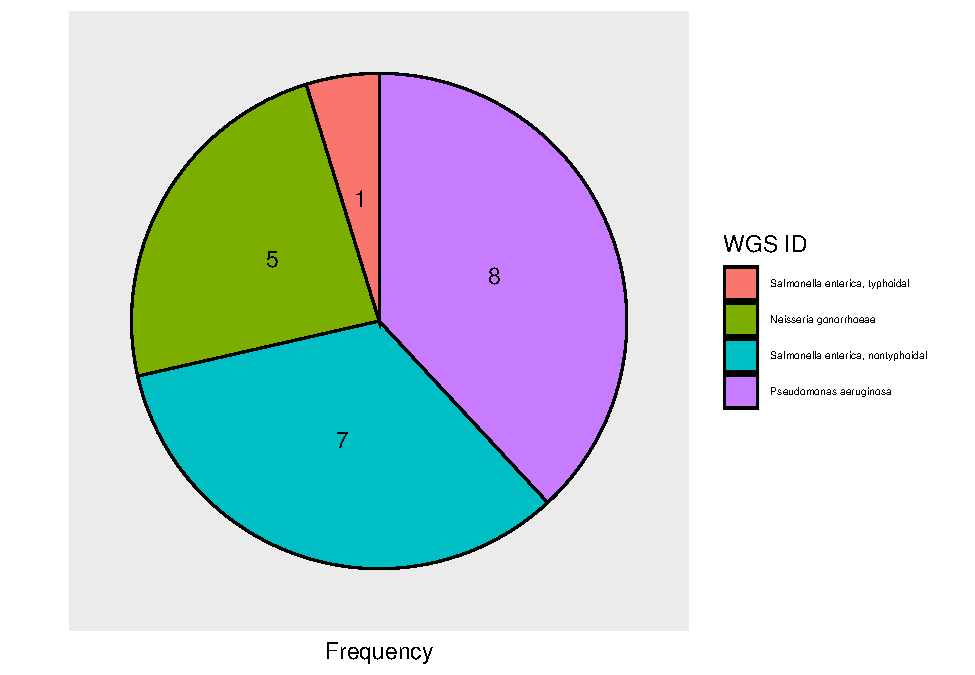
\includegraphics[keepaspectratio]{qualifyr_report_2025-06-20_A_files/figure-latex/pie_chart-1.pdf}}

\subsubsection{Result Classification}\label{result-classification}

\pandocbounded{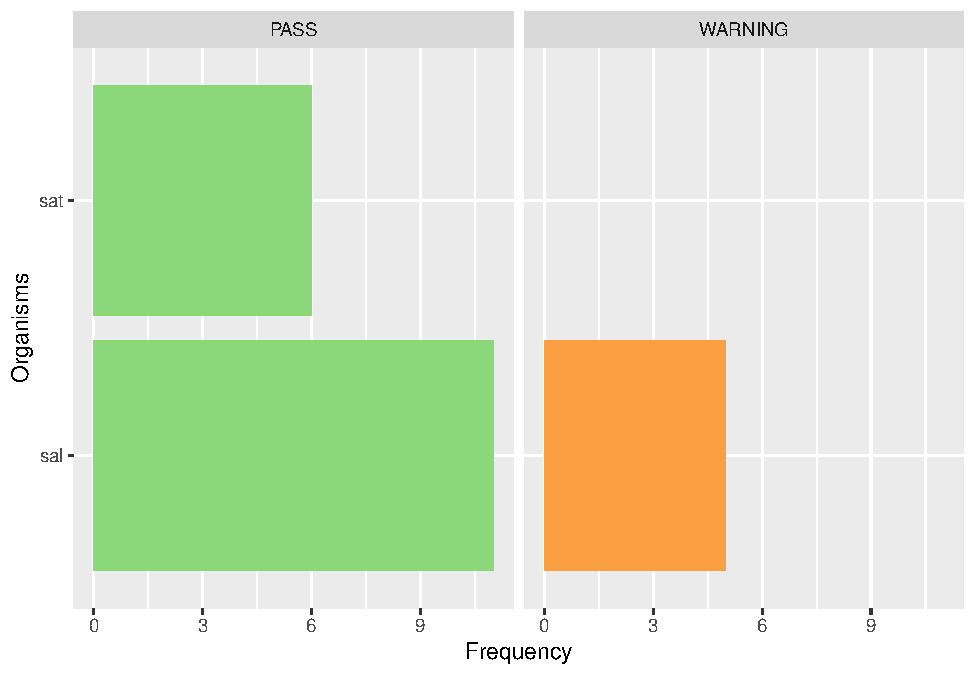
\includegraphics[keepaspectratio]{qualifyr_report_2025-06-20_A_files/figure-latex/organism results-1.pdf}}

\subsubsection{Number of contigs}\label{number-of-contigs}

\pandocbounded{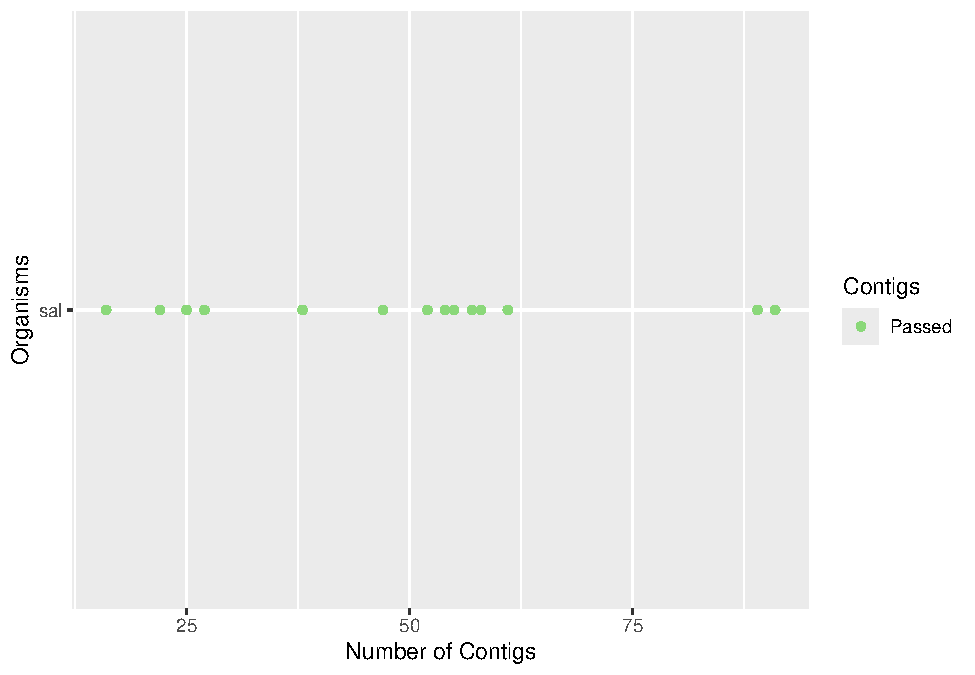
\includegraphics[keepaspectratio]{qualifyr_report_2025-06-20_A_files/figure-latex/unnamed-chunk-1-1.pdf}}

\subsubsection{N50 Value}\label{n50-value}

\pandocbounded{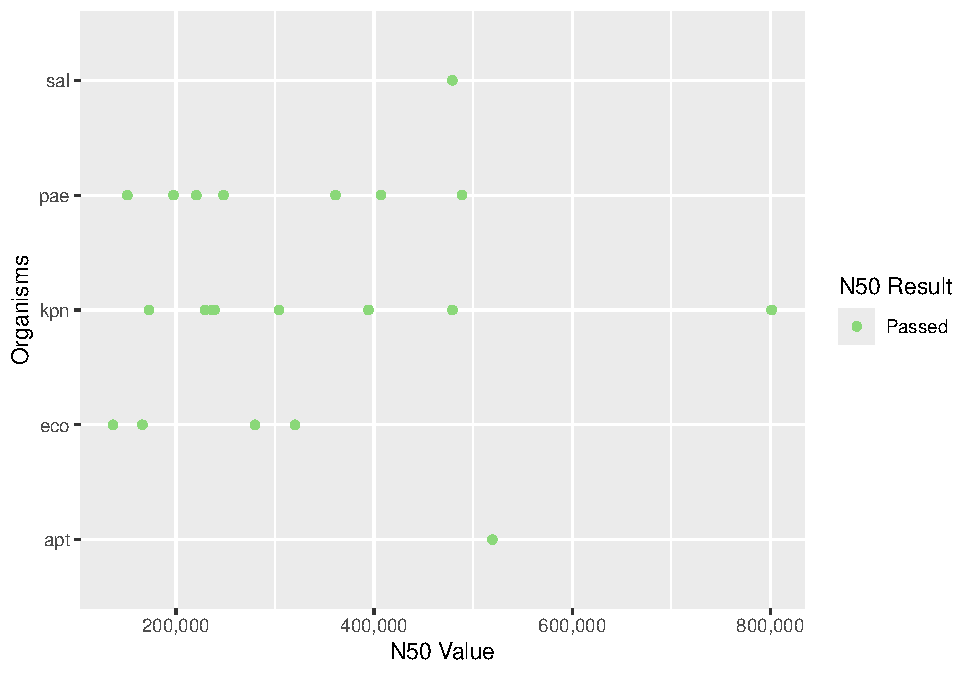
\includegraphics[keepaspectratio]{qualifyr_report_2025-06-20_A_files/figure-latex/n50_result -1.pdf}}

\subsubsection{Total Length}\label{total-length}

\pandocbounded{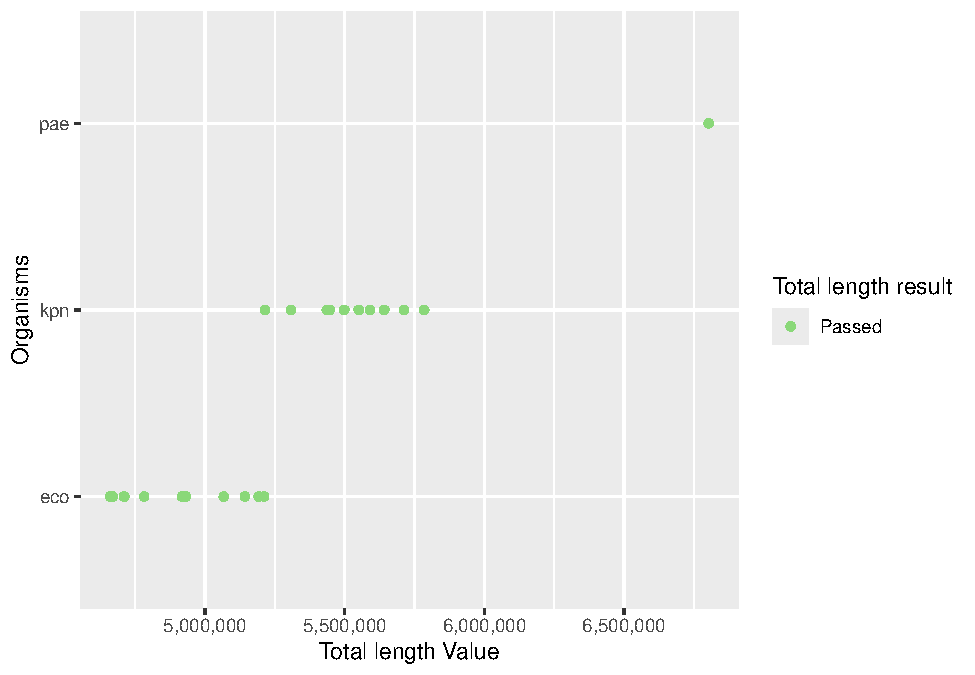
\includegraphics[keepaspectratio]{qualifyr_report_2025-06-20_A_files/figure-latex/length_result -1.pdf}}

\fontsize{7}{8}
\selectfont
\captionsetup[table]{labelformat=empty}
\renewcommand{\arraystretch}{1}

\subsubsection{MLST RESULTS}\label{mlst-results}

\begin{longtable}[l]{>{\centering\arraybackslash}p{3cm}>{\centering\arraybackslash}p{3cm}>{\centering\arraybackslash}p{1cm}>{\centering\arraybackslash}p{1cm}>{\centering\arraybackslash}p{1cm}>{\centering\arraybackslash}p{1cm}>{\centering\arraybackslash}p{1cm}>{\centering\arraybackslash}p{1cm}>{\centering\arraybackslash}p{1cm}>{\centering\arraybackslash}p{1cm}}
\toprule
\cellcolor[HTML]{D4D4D4}{\textbf{sample\_id}} & \cellcolor[HTML]{D4D4D4}{\textbf{species}} & \cellcolor[HTML]{D4D4D4}{\textbf{MLST}} & \cellcolor[HTML]{D4D4D4}{\textbf{gapA}} & \cellcolor[HTML]{D4D4D4}{\textbf{infB}} & \cellcolor[HTML]{D4D4D4}{\textbf{mdh}} & \cellcolor[HTML]{D4D4D4}{\textbf{pgi}} & \cellcolor[HTML]{D4D4D4}{\textbf{phoE}} & \cellcolor[HTML]{D4D4D4}{\textbf{rpoB}} & \cellcolor[HTML]{D4D4D4}{\textbf{tonB}}\\
\midrule
24ARS\_BRH0191 & \em{Klebsiella pneumoniae} & 23 & 2 & 1 & 1 & 1 & 9 & 4 & 12\\
24ARS\_BRH0192 & \em{Klebsiella pneumoniae} & 2385 & 2 & 1 & 65 & 2 & 5 & 1 & 350\\
24ARS\_BRH0195 & \em{Klebsiella pneumoniae} & 147 & 3 & 4 & 6 & 1 & 7 & 4 & 38\\
24ARS\_CRH0210 & \em{Klebsiella pneumoniae} & 101 & 2 & 6 & 1 & 5 & 4 & 1 & 6\\
24ARS\_DMC0490 & \em{Klebsiella pneumoniae} & 3113 & 31 & 1 & 1 & 1 & 3 & 1 & 64\\
\addlinespace
24ARS\_DMC0492 & \em{Klebsiella pneumoniae} & 5605 & 2 & 6 & 17 & 368 & 20 & 10 & 25\\
24ARS\_DMC0494 & \em{Klebsiella pneumoniae} & 29 & 2 & 3 & 2 & 2 & 6 & 4 & 4\\
24ARS\_GMH0269 & \em{Klebsiella pneumoniae} & 2050 & 2 & 3 & 2 & 37 & 10 & 1 & 15\\
24ARS\_GMH0281 & \em{Klebsiella pneumoniae} & 147 & 3 & 4 & 6 & 1 & 7 & 4 & 38\\
24ARS\_JLM0247 & \em{Klebsiella pneumoniae} & 23 & 2 & 1 & 1 & 1 & 9 & 4 & 12\\
\addlinespace
24ARS\_JLM0248 & \em{Klebsiella pneumoniae} & 592 & 2 & 3 & 6 & 1 & 9 & 4 & 13\\
24ARS\_MAR0317 & \em{Klebsiella pneumoniae} & 101 & 2 & 6 & 1 & 5 & 4 & 1 & 6\\
24ARS\_NKI0075 & \em{Klebsiella pneumoniae} & - & 2 & 5 & 1 & 1 & 14 & 3 & 20\\
24ARS\_NKI0077 & \em{Klebsiella quasipneumoniae} & - & 18 & 22 & 55 & 109 & 114 & 91 & 51\\
24ARS\_VSM0556 & \em{Klebsiella pneumoniae} & 147 & 3 & 4 & 6 & 1 & 7 & 4 & 38\\
\addlinespace
24ARS\_VSM0557 & \em{Klebsiella pneumoniae} & 86 & 9 & 4 & 2 & 1 & 1 & 1 & 27\\
24ARS\_VSM0586 & \em{Klebsiella pneumoniae} & 147 & 3 & 4 & 6 & 1 & 7 & 4 & 38\\
24ARS\_VSM0660 & \em{Klebsiella pneumoniae} & 37 & 2 & 9 & 2 & 1 & 13 & 1 & 16\\
24ARS\_VSM0662 & \em{Klebsiella pneumoniae} & 11 & 3 & 3 & 1 & 1 & 1 & 1 & 4\\
25ARS\_DMC0010 & \em{Klebsiella pneumoniae} & 147 & 3 & 4 & 6 & 1 & 7 & 4 & 38\\
\addlinespace
25ARS\_GMH0007 & \em{Klebsiella pneumoniae} & 147 & 3 & 4 & 6 & 1 & 7 & 4 & 38\\
25ARS\_MAR0014 & \em{Klebsiella pneumoniae} & 39 & 2 & 1 & 2 & 4 & 9 & 1 & 14\\
\bottomrule
\multicolumn{10}{l}{\rule{0pt}{1em}\textit{Legend: } (-) Not identified}\\
\end{longtable}

\subsubsection{MLST RESULTS SUMMARY:}\label{mlst-results-summary}

\begin{longtable}[l]{>{\raggedright\arraybackslash}p{6cm}>{\raggedright\arraybackslash}p{10cm}}
\toprule
\cellcolor[HTML]{D4D4D4}{\textbf{wgs\_id}} & \cellcolor[HTML]{D4D4D4}{\textbf{mlst\_count}}\\
\midrule
\em{Klebsiella pneumoniae} & 23 (n= 2 ), 2385 (n= 1 ), 147 (n= 6 ), 101 (n= 2 ), 3113 (n= 1 ), 5605 (n= 1 ), 29 (n= 1 ), 2050 (n= 1 ), 592 (n= 1 ), - (n= 1 ), 86 (n= 1 ), 37 (n= 1 ), 11 (n= 1 ), 39 (n= 1 )\\
\em{Klebsiella quasipneumoniae} & - (n= 1 )\\
\bottomrule
\multicolumn{2}{l}{\rule{0pt}{1em}\textit{Legend: } (-) Not identified}\\
\end{longtable}

\newpage
\begin{landscape}
\fontsize{7}{8}
\selectfont
\captionsetup[table]{labelformat=empty}
\renewcommand{\arraystretch}{1.2}


\normalsize\textbf{AMR PREDICTION RESULTS}\textbf\normalsize




\fontsize{7}{8}
\selectfont
\captionsetup[table]{labelformat=empty}
\renewcommand{\arraystretch}{1.2}

\begingroup\fontsize{7}{9}\selectfont

\resizebox{\ifdim\width>\linewidth\linewidth\else\width\fi}{!}{
\begin{tabular}{c>{\centering\arraybackslash}p{3cm}>{\centering\arraybackslash}p{3cm}>{\centering\arraybackslash}p{3cm}>{\centering\arraybackslash}p{3cm}>{\centering\arraybackslash}p{3cm}>{\centering\arraybackslash}p{3cm}}
\toprule
\multicolumn{7}{l}{\textbf{\textit{Klebsiella pneumoniae} (Part 1.1)}} \\
\cmidrule(l{3pt}r{3pt}){1-7}
\cellcolor[HTML]{D4D4D4}{\textbf{sample\_id}} & \cellcolor[HTML]{D4D4D4}{\textbf{AMR AMIKACIN/ KAMYCIN}} & \cellcolor[HTML]{D4D4D4}{\textbf{AMR AMIKACIN/ KAMYCIN/ QUINOLONE/ TOBRAMYCIN}} & \cellcolor[HTML]{D4D4D4}{\textbf{AMR AMINOGLYCOSIDE}} & \cellcolor[HTML]{D4D4D4}{\textbf{AMR AZITHROMYCIN/ ERYTHROMYCIN/ SPIRAMYCIN/ TELITHROMYCIN}} & \cellcolor[HTML]{D4D4D4}{\textbf{AMR BETA-LACTAM}} & \cellcolor[HTML]{D4D4D4}{\textbf{AMR BLEOMYCIN}}\\
\midrule
24ARS\_BRH0191 & NA & NA & NA & NA & blaSHV-11 & NA\\
24ARS\_BRH0192 & NA & NA & NA & NA & blaSHV-75 & NA\\
24ARS\_BRH0195 & NA & aac(6')-Ib-cr5 & NA & mph(A) & blaTEM-1, blaSHV-11 & ble\\
24ARS\_CRH0210 & NA & NA & rmtB1 & mph(A) & blaSHV-1, blaTEM-1 & ble\\
24ARS\_DMC0490 & NA & aac(6')-Ib-cr5 & NA & mph(A) & blaTEM-1, blaSHV-220 & NA\\
\addlinespace
24ARS\_DMC0492 & NA & NA & NA & NA & blaSHV-32 & NA\\
\bottomrule
\end{tabular}}
\endgroup{}


\vspace{5mm}

\begingroup\fontsize{7}{9}\selectfont

\resizebox{\ifdim\width>\linewidth\linewidth\else\width\fi}{!}{
\begin{tabular}{c>{\centering\arraybackslash}p{3cm}>{\centering\arraybackslash}p{3cm}>{\centering\arraybackslash}p{3cm}>{\centering\arraybackslash}p{3cm}>{\centering\arraybackslash}p{3cm}>{\centering\arraybackslash}p{3cm}}
\toprule
\multicolumn{7}{l}{\textbf{\textit{Klebsiella pneumoniae} (Part 1.2)}} \\
\cmidrule(l{3pt}r{3pt}){1-7}
\cellcolor[HTML]{D4D4D4}{\textbf{sample\_id}} & \cellcolor[HTML]{D4D4D4}{\textbf{AMR CARBAPENEM}} & \cellcolor[HTML]{D4D4D4}{\textbf{AMR CEPHALOSPORIN}} & \cellcolor[HTML]{D4D4D4}{\textbf{AMR CHLORAMPHENICOL}} & \cellcolor[HTML]{D4D4D4}{\textbf{AMR CHLORAMPHENICOL/ FLORFENICOL}} & \cellcolor[HTML]{D4D4D4}{\textbf{AMR CLINDAMYCIN/ ERYTHROMYCIN}} & \cellcolor[HTML]{D4D4D4}{\textbf{AMR CLINDAMYCIN/ ERYTHROMYCIN/ STREPTOGRAMIN B}}\\
\midrule
24ARS\_BRH0191 & NA & NA & NA & NA & NA & NA\\
24ARS\_BRH0192 & NA & NA & NA & NA & NA & NA\\
24ARS\_BRH0195 & blaNDM-7 & blaOXA-10, blaCTX-M-15, blaOXA-1 & cmlA5, catB3 & floR & erm(42) & NA\\
24ARS\_CRH0210 & blaNDM-5 & blaCTX-M-15 & NA & NA & NA & erm(B)\\
24ARS\_DMC0490 & NA & blaCTX-M-15 & NA & NA & NA & NA\\
\addlinespace
24ARS\_DMC0492 & NA & NA & NA & NA & NA & NA\\
\bottomrule
\end{tabular}}
\endgroup{}


\vspace{5mm}

\begingroup\fontsize{7}{9}\selectfont

\resizebox{\ifdim\width>\linewidth\linewidth\else\width\fi}{!}{
\begin{tabular}{c>{\centering\arraybackslash}p{3cm}>{\centering\arraybackslash}p{3cm}>{\centering\arraybackslash}p{3cm}>{\centering\arraybackslash}p{3cm}>{\centering\arraybackslash}p{3cm}>{\centering\arraybackslash}p{3cm}}
\toprule
\multicolumn{7}{l}{\textbf{\textit{Klebsiella pneumoniae} (Part 1.3)}} \\
\cmidrule(l{3pt}r{3pt}){1-7}
\cellcolor[HTML]{D4D4D4}{\textbf{sample\_id}} & \cellcolor[HTML]{D4D4D4}{\textbf{AMR EFFLUX}} & \cellcolor[HTML]{D4D4D4}{\textbf{AMR FOSFOMYCIN}} & \cellcolor[HTML]{D4D4D4}{\textbf{AMR GENTAMICIN}} & \cellcolor[HTML]{D4D4D4}{\textbf{AMR KAMYCIN}} & \cellcolor[HTML]{D4D4D4}{\textbf{AMR PHENICOL/ QUINOLONE}} & \cellcolor[HTML]{D4D4D4}{\textbf{AMR QUINOLONE}}\\
\midrule
24ARS\_BRH0191 & kdeA, emrD & fosA & NA & NA & oqxB19, oqxA & NA\\
24ARS\_BRH0192 & emrD, kdeA & fosA & NA & NA & oqxB19, oqxA & NA\\
24ARS\_BRH0195 & kdeA, emrD & fosA & NA & aph(3')-Ia & oqxA, oqxB & qnrS1, qnrB1\\
24ARS\_CRH0210 & kdeA, emrD & fosA & NA & NA & oqxA, oqxB20 & NA\\
24ARS\_DMC0490 & emrD, kdeA & fosA & NA & NA & oqxB32, oqxA & qnrB6, qnrS1\\
\addlinespace
24ARS\_DMC0492 & emrD, kdeA & fosA & NA & NA & oqxA10, oqxB & NA\\
\bottomrule
\end{tabular}}
\endgroup{}


\vspace{5mm}

\begingroup\fontsize{7}{9}\selectfont

\resizebox{\ifdim\width>\linewidth\linewidth\else\width\fi}{!}{
\begin{tabular}{c>{\centering\arraybackslash}p{3cm}>{\centering\arraybackslash}p{3cm}>{\centering\arraybackslash}p{3cm}>{\centering\arraybackslash}p{3cm}>{\centering\arraybackslash}p{3cm}>{\centering\arraybackslash}p{3cm}}
\toprule
\multicolumn{7}{l}{\textbf{\textit{Klebsiella pneumoniae} (Part 1.4)}} \\
\cmidrule(l{3pt}r{3pt}){1-7}
\cellcolor[HTML]{D4D4D4}{\textbf{sample\_id}} & \cellcolor[HTML]{D4D4D4}{\textbf{AMR RIFAMYCIN}} & \cellcolor[HTML]{D4D4D4}{\textbf{AMR STREPTOMYCIN}} & \cellcolor[HTML]{D4D4D4}{\textbf{AMR SULFOMIDE}} & \cellcolor[HTML]{D4D4D4}{\textbf{AMR TETRACYCLINE}} & \cellcolor[HTML]{D4D4D4}{\textbf{AMR TRIMETHOPRIM}} & \cellcolor[HTML]{D4D4D4}{\textbf{STRESS }}\\
\midrule
24ARS\_BRH0191 & NA & NA & NA & NA & NA & fieF, asr\\
24ARS\_BRH0192 & NA & NA & NA & NA & NA & fieF, asr\\
24ARS\_BRH0195 & arr-2 & aadA1, aph(6)-Id, aph(3'')-Ib & sul1, sul2 & NA & dfrA14 & fieF\\
24ARS\_CRH0210 & NA & aadA2 & sul1 & NA & dfrA12 & fieF\\
24ARS\_DMC0490 & arr-3 & aadA16 & sul1 & NA & dfrA27 & fieF, asr, psi-GI, kefB-GI, trxLHR, hdeD-GI, yfdX2, yfdX1, shsP, clpK, hsp20\\
\addlinespace
24ARS\_DMC0492 & NA & NA & NA & NA & NA & fieF\\
\bottomrule
\end{tabular}}
\endgroup{}


\vspace{5mm}

\begingroup\fontsize{7}{9}\selectfont

\resizebox{\ifdim\width>\linewidth\linewidth\else\width\fi}{!}{
\begin{tabular}{c>{\centering\arraybackslash}p{3cm}>{\centering\arraybackslash}p{3cm}>{\centering\arraybackslash}p{3cm}>{\centering\arraybackslash}p{3cm}>{\centering\arraybackslash}p{3cm}>{\centering\arraybackslash}p{3cm}}
\toprule
\multicolumn{7}{l}{\textbf{\textit{Klebsiella pneumoniae} (Part 1.5)}} \\
\cmidrule(l{3pt}r{3pt}){1-7}
\cellcolor[HTML]{D4D4D4}{\textbf{sample\_id}} & \cellcolor[HTML]{D4D4D4}{\textbf{STRESS ARSENIC}} & \cellcolor[HTML]{D4D4D4}{\textbf{STRESS ARSENITE}} & \cellcolor[HTML]{D4D4D4}{\textbf{STRESS ARSETE}} & \cellcolor[HTML]{D4D4D4}{\textbf{STRESS COPPER}} & \cellcolor[HTML]{D4D4D4}{\textbf{STRESS COPPER/ SILVER}} & \cellcolor[HTML]{D4D4D4}{\textbf{STRESS FLUORIDE}}\\
\midrule
24ARS\_BRH0191 & NA & NA & arsC & pcoS, pcoR, pcoD, pcoC, pcoB, pcoA & silA, silB, silF, silC, silR, silS & NA\\
24ARS\_BRH0192 & NA & NA & NA & NA & silC, silF, silS, silR & NA\\
24ARS\_BRH0195 & NA & NA & arsC & NA & NA & NA\\
24ARS\_CRH0210 & NA & NA & arsC & NA & NA & NA\\
24ARS\_DMC0490 & arsR & arsB, arsA, arsD & arsC, arsC, arsC & pcoS, pcoR, pcoD, pcoC, pcoB, pcoA & silA, silB, silF, silC, silR, silS & NA\\
\addlinespace
24ARS\_DMC0492 & NA & NA & arsC & NA & NA & NA\\
\bottomrule
\end{tabular}}
\endgroup{}


\vspace{5mm}

\begingroup\fontsize{7}{9}\selectfont

\resizebox{\ifdim\width>\linewidth\linewidth\else\width\fi}{!}{
\begin{tabular}{c>{\centering\arraybackslash}p{3cm}>{\centering\arraybackslash}p{3cm}>{\centering\arraybackslash}p{3cm}>{\centering\arraybackslash}p{3cm}>{\centering\arraybackslash}p{3cm}>{\centering\arraybackslash}p{3cm}}
\toprule
\multicolumn{7}{l}{\textbf{\textit{Klebsiella pneumoniae} (Part 1.6)}} \\
\cmidrule(l{3pt}r{3pt}){1-7}
\cellcolor[HTML]{D4D4D4}{\textbf{sample\_id}} & \cellcolor[HTML]{D4D4D4}{\textbf{STRESS MERCURY}} & \cellcolor[HTML]{D4D4D4}{\textbf{STRESS ORGANOMERCURY}} & \cellcolor[HTML]{D4D4D4}{\textbf{STRESS QUATERRY AMMONIUM}} & \cellcolor[HTML]{D4D4D4}{\textbf{STRESS SILVER}} & \cellcolor[HTML]{D4D4D4}{\textbf{STRESS TELLURIUM}} & \cellcolor[HTML]{D4D4D4}{\textbf{VIRULENCE }}\\
\midrule
24ARS\_BRH0191 & NA & NA & NA & silP & terB, terC, terD, terE & rmpD, rmpC, rmpA2, iutA, iucC, iucB, iucA, rmpA, iroC, peg-344, iroN, iroD, ybtP, iroB, mchF, ybtQ\\
24ARS\_BRH0192 & NA & NA & NA & NA & terE, terD, terC, terB & iroN, iroD, ybtP, ybtQ, iroB, iroC, peg-344, rmpC, rmpD, rmpA, iutA, iucC, iucB, iucA\\
24ARS\_BRH0195 & merE, merD, merA, merP, merT, merR & merC & qacEdelta1 & NA & NA & NA\\
24ARS\_CRH0210 & NA & NA & qacEdelta1 & NA & NA & ybtQ, ybtP\\
24ARS\_DMC0490 & NA & NA & qacEdelta1 & silP, silE & NA & NA\\
\addlinespace
24ARS\_DMC0492 & NA & NA & NA & NA & NA & NA\\
\bottomrule
\end{tabular}}
\endgroup{}


\vspace{10mm}

\begingroup\fontsize{7}{9}\selectfont

\resizebox{\ifdim\width>\linewidth\linewidth\else\width\fi}{!}{
\begin{tabular}{l>{\centering\arraybackslash}p{3cm}>{\centering\arraybackslash}p{3cm}>{\centering\arraybackslash}p{3cm}>{\centering\arraybackslash}p{3cm}>{\centering\arraybackslash}p{3cm}>{\centering\arraybackslash}p{3cm}c}
\toprule
\multicolumn{7}{l}{\textbf{\textit{Klebsiella pneumoniae} (Part 2.1)}} \\
\cmidrule(l{3pt}r{3pt}){1-7}
\cellcolor[HTML]{D4D4D4}{\textbf{ }} & \cellcolor[HTML]{D4D4D4}{\textbf{sample\_id}} & \cellcolor[HTML]{D4D4D4}{\textbf{AMR AMIKACIN/ KAMYCIN}} & \cellcolor[HTML]{D4D4D4}{\textbf{AMR AMIKACIN/ KAMYCIN/ QUINOLONE/ TOBRAMYCIN}} & \cellcolor[HTML]{D4D4D4}{\textbf{AMR AMINOGLYCOSIDE}} & \cellcolor[HTML]{D4D4D4}{\textbf{AMR AZITHROMYCIN/ ERYTHROMYCIN/ SPIRAMYCIN/ TELITHROMYCIN}} & \cellcolor[HTML]{D4D4D4}{\textbf{AMR BETA-LACTAM}} & \cellcolor[HTML]{D4D4D4}{\textbf{AMR BLEOMYCIN}}\\
\midrule
7 & 24ARS\_DMC0494 & NA & NA & NA & NA & blaTEM-1 & NA\\
8 & 24ARS\_GMH0269 & NA & NA & NA & NA & blaSHV-1 & NA\\
9 & 24ARS\_GMH0281 & aph(3')-VI & aac(6')-Ib-cr5 & NA & mph(A) & blaSHV-11, blaTEM-1 & ble\\
10 & 24ARS\_JLM0247 & NA & NA & NA & NA & blaSHV-11 & NA\\
11 & 24ARS\_JLM0248 & NA & NA & NA & NA & blaSHV-26 & NA\\
\addlinespace
12 & 24ARS\_MAR0317 & NA & aac(6')-Ib-cr5 & rmtB1 & mph(A) & blaSHV-1, blaTEM-1 & ble\\
\bottomrule
\end{tabular}}
\endgroup{}


\vspace{5mm}

\begingroup\fontsize{7}{9}\selectfont

\resizebox{\ifdim\width>\linewidth\linewidth\else\width\fi}{!}{
\begin{tabular}{l>{\centering\arraybackslash}p{3cm}>{\centering\arraybackslash}p{3cm}>{\centering\arraybackslash}p{3cm}>{\centering\arraybackslash}p{3cm}>{\centering\arraybackslash}p{3cm}>{\centering\arraybackslash}p{3cm}c}
\toprule
\multicolumn{7}{l}{\textbf{\textit{Klebsiella pneumoniae} (Part 2.2)}} \\
\cmidrule(l{3pt}r{3pt}){1-7}
\cellcolor[HTML]{D4D4D4}{\textbf{ }} & \cellcolor[HTML]{D4D4D4}{\textbf{sample\_id}} & \cellcolor[HTML]{D4D4D4}{\textbf{AMR CARBAPENEM}} & \cellcolor[HTML]{D4D4D4}{\textbf{AMR CEPHALOSPORIN}} & \cellcolor[HTML]{D4D4D4}{\textbf{AMR CHLORAMPHENICOL}} & \cellcolor[HTML]{D4D4D4}{\textbf{AMR CHLORAMPHENICOL/ FLORFENICOL}} & \cellcolor[HTML]{D4D4D4}{\textbf{AMR CLINDAMYCIN/ ERYTHROMYCIN}} & \cellcolor[HTML]{D4D4D4}{\textbf{AMR CLINDAMYCIN/ ERYTHROMYCIN/ STREPTOGRAMIN B}}\\
\midrule
7 & 24ARS\_DMC0494 & NA & blaSHV-187, blaCTX-M-15 & NA & NA & NA & NA\\
8 & 24ARS\_GMH0269 & NA & NA & NA & NA & NA & NA\\
9 & 24ARS\_GMH0281 & blaNDM-1 & blaCTX-M-15, blaOXA-1, blaOXA-10 & cmlA5, catB3 & floR & erm(42) & NA\\
10 & 24ARS\_JLM0247 & NA & NA & NA & NA & NA & NA\\
11 & 24ARS\_JLM0248 & NA & NA & NA & NA & NA & NA\\
\addlinespace
12 & 24ARS\_MAR0317 & blaNDM-5 & blaCTX-M-15, blaOXA-1 & catB3 & NA & NA & erm(B)\\
\bottomrule
\end{tabular}}
\endgroup{}


\vspace{5mm}

\begingroup\fontsize{7}{9}\selectfont

\resizebox{\ifdim\width>\linewidth\linewidth\else\width\fi}{!}{
\begin{tabular}{l>{\centering\arraybackslash}p{3cm}>{\centering\arraybackslash}p{3cm}>{\centering\arraybackslash}p{3cm}>{\centering\arraybackslash}p{3cm}>{\centering\arraybackslash}p{3cm}>{\centering\arraybackslash}p{3cm}c}
\toprule
\multicolumn{7}{l}{\textbf{\textit{Klebsiella pneumoniae} (Part 2.3)}} \\
\cmidrule(l{3pt}r{3pt}){1-7}
\cellcolor[HTML]{D4D4D4}{\textbf{ }} & \cellcolor[HTML]{D4D4D4}{\textbf{sample\_id}} & \cellcolor[HTML]{D4D4D4}{\textbf{AMR EFFLUX}} & \cellcolor[HTML]{D4D4D4}{\textbf{AMR FOSFOMYCIN}} & \cellcolor[HTML]{D4D4D4}{\textbf{AMR GENTAMICIN}} & \cellcolor[HTML]{D4D4D4}{\textbf{AMR KAMYCIN}} & \cellcolor[HTML]{D4D4D4}{\textbf{AMR PHENICOL/ QUINOLONE}} & \cellcolor[HTML]{D4D4D4}{\textbf{AMR QUINOLONE}}\\
\midrule
7 & 24ARS\_DMC0494 & emrD, kdeA & fosA & NA & NA & oqxB25, oqxA & qnrB1\\
8 & 24ARS\_GMH0269 & kdeA, emrD & fosA & NA & NA & oqxB25, oqxA & NA\\
9 & 24ARS\_GMH0281 & kdeA, emrD & fosA & NA & aph(3')-Ia & oqxB, oqxA & NA\\
10 & 24ARS\_JLM0247 & kdeA, emrD & fosA & NA & NA & oqxB19, oqxA & NA\\
11 & 24ARS\_JLM0248 & kdeA, emrD & fosA & NA & NA & oqxA10, oqxB & NA\\
\addlinespace
12 & 24ARS\_MAR0317 & emrD, kdeA & fosA & NA & NA & NA & NA\\
\bottomrule
\end{tabular}}
\endgroup{}


\vspace{5mm}

\begingroup\fontsize{7}{9}\selectfont

\resizebox{\ifdim\width>\linewidth\linewidth\else\width\fi}{!}{
\begin{tabular}{l>{\centering\arraybackslash}p{3cm}>{\centering\arraybackslash}p{3cm}>{\centering\arraybackslash}p{3cm}>{\centering\arraybackslash}p{3cm}>{\centering\arraybackslash}p{3cm}>{\centering\arraybackslash}p{3cm}c}
\toprule
\multicolumn{7}{l}{\textbf{\textit{Klebsiella pneumoniae} (Part 2.4)}} \\
\cmidrule(l{3pt}r{3pt}){1-7}
\cellcolor[HTML]{D4D4D4}{\textbf{ }} & \cellcolor[HTML]{D4D4D4}{\textbf{sample\_id}} & \cellcolor[HTML]{D4D4D4}{\textbf{AMR RIFAMYCIN}} & \cellcolor[HTML]{D4D4D4}{\textbf{AMR STREPTOMYCIN}} & \cellcolor[HTML]{D4D4D4}{\textbf{AMR SULFOMIDE}} & \cellcolor[HTML]{D4D4D4}{\textbf{AMR TETRACYCLINE}} & \cellcolor[HTML]{D4D4D4}{\textbf{AMR TRIMETHOPRIM}} & \cellcolor[HTML]{D4D4D4}{\textbf{STRESS }}\\
\midrule
7 & 24ARS\_DMC0494 & NA & aph(6)-Id, aph(3'')-Ib & sul2 & NA & dfrA14 & asr, fieF\\
8 & 24ARS\_GMH0269 & NA & NA & NA & tet(A) & NA & fieF, asr\\
9 & 24ARS\_GMH0281 & arr-2 & aadA1, aph(3'')-Ib, aph(6)-Id & sul2 & NA & dfrA14 & fieF\\
10 & 24ARS\_JLM0247 & NA & NA & NA & NA & NA & asr, fieF\\
11 & 24ARS\_JLM0248 & NA & NA & NA & NA & NA & asr, fieF\\
\addlinespace
12 & 24ARS\_MAR0317 & NA & aph(3'')-Ib, aph(6)-Id & sul1, sul2 & tet(A) & dfrA14 & fieF\\
\bottomrule
\end{tabular}}
\endgroup{}


\vspace{5mm}

\begingroup\fontsize{7}{9}\selectfont

\resizebox{\ifdim\width>\linewidth\linewidth\else\width\fi}{!}{
\begin{tabular}{l>{\centering\arraybackslash}p{3cm}>{\centering\arraybackslash}p{3cm}>{\centering\arraybackslash}p{3cm}>{\centering\arraybackslash}p{3cm}>{\centering\arraybackslash}p{3cm}>{\centering\arraybackslash}p{3cm}c}
\toprule
\multicolumn{7}{l}{\textbf{\textit{Klebsiella pneumoniae} (Part 2.5)}} \\
\cmidrule(l{3pt}r{3pt}){1-7}
\cellcolor[HTML]{D4D4D4}{\textbf{ }} & \cellcolor[HTML]{D4D4D4}{\textbf{sample\_id}} & \cellcolor[HTML]{D4D4D4}{\textbf{STRESS ARSENIC}} & \cellcolor[HTML]{D4D4D4}{\textbf{STRESS ARSENITE}} & \cellcolor[HTML]{D4D4D4}{\textbf{STRESS ARSETE}} & \cellcolor[HTML]{D4D4D4}{\textbf{STRESS COPPER}} & \cellcolor[HTML]{D4D4D4}{\textbf{STRESS COPPER/ SILVER}} & \cellcolor[HTML]{D4D4D4}{\textbf{STRESS FLUORIDE}}\\
\midrule
7 & 24ARS\_DMC0494 & arsR & arsD, arsA, arsB & arsC, arsC & pcoE, pcoS, pcoR, pcoD, pcoC, pcoB, pcoA & silA, silB, silF, silC, silR, silS & NA\\
8 & 24ARS\_GMH0269 & NA & NA & arsC & pcoS, pcoA, pcoB, pcoC, pcoD, pcoR & silS, silR, silC, silF, silB, silA & NA\\
9 & 24ARS\_GMH0281 & arsR & arsD, arsA, arsB & arsC, arsC & pcoE, pcoS, pcoR, pcoD, pcoC, pcoB, pcoA & silA, silB, silF, silC, silR, silS & NA\\
10 & 24ARS\_JLM0247 & NA & NA & arsC & pcoA, pcoB, pcoC, pcoD, pcoR, pcoS & silF, silC, silB, silA, silR, silS & NA\\
11 & 24ARS\_JLM0248 & NA & NA & arsC & pcoR, pcoD, pcoS, pcoC, pcoB, pcoA & silS, silR, silA, silB, silC & NA\\
\addlinespace
12 & 24ARS\_MAR0317 & arsR & arsD, arsA, arsB & arsC, arsC & pcoS, pcoA, pcoB, pcoC, pcoD, pcoR & silS, silR, silC, silF, silB, silA & NA\\
\bottomrule
\end{tabular}}
\endgroup{}


\vspace{5mm}

\begingroup\fontsize{7}{9}\selectfont

\resizebox{\ifdim\width>\linewidth\linewidth\else\width\fi}{!}{
\begin{tabular}{l>{\centering\arraybackslash}p{3cm}>{\centering\arraybackslash}p{3cm}>{\centering\arraybackslash}p{3cm}>{\centering\arraybackslash}p{3cm}>{\centering\arraybackslash}p{3cm}>{\centering\arraybackslash}p{3cm}c}
\toprule
\multicolumn{7}{l}{\textbf{\textit{Klebsiella pneumoniae} (Part 2.6)}} \\
\cmidrule(l{3pt}r{3pt}){1-7}
\cellcolor[HTML]{D4D4D4}{\textbf{ }} & \cellcolor[HTML]{D4D4D4}{\textbf{sample\_id}} & \cellcolor[HTML]{D4D4D4}{\textbf{STRESS MERCURY}} & \cellcolor[HTML]{D4D4D4}{\textbf{STRESS ORGANOMERCURY}} & \cellcolor[HTML]{D4D4D4}{\textbf{STRESS QUATERRY AMMONIUM}} & \cellcolor[HTML]{D4D4D4}{\textbf{STRESS SILVER}} & \cellcolor[HTML]{D4D4D4}{\textbf{STRESS TELLURIUM}} & \cellcolor[HTML]{D4D4D4}{\textbf{VIRULENCE }}\\
\midrule
7 & 24ARS\_DMC0494 & NA & NA & NA & silP, silE & NA & ybtQ, ybtP\\
8 & 24ARS\_GMH0269 & NA & NA & NA & NA & terE, terC, terB, terD & ybtP, ybtQ, rmpA, rmpD, rmpC, peg-344, iroN, iroD, iroC, iroB, iucA, iucB, iucC, iutA\\
9 & 24ARS\_GMH0281 & NA & NA & NA & silP, silE & terE, terD, terC, terB & NA\\
10 & 24ARS\_JLM0247 & NA & NA & NA & silP & terB, terC, terD, terE & rmpA2, rmpA, rmpD, rmpC, peg-344, iroN, iroD, iroC, iroB, ybtP, iucA, mchF, ybtQ, iucB, iutA\\
11 & 24ARS\_JLM0248 & NA & NA & NA & silP, silE & terB, terC, terD, terE & rmpA, rmpD, rmpC, peg-344, iroN, iroD, iroC, iroB, iucA, iucB, iucC, iutA\\
\addlinespace
12 & 24ARS\_MAR0317 & NA & NA & qacEdelta1 & silE, silP & NA & ybtP, ybtQ\\
\bottomrule
\end{tabular}}
\endgroup{}


\vspace{10mm}

\begingroup\fontsize{7}{9}\selectfont

\resizebox{\ifdim\width>\linewidth\linewidth\else\width\fi}{!}{
\begin{tabular}{l>{\centering\arraybackslash}p{3cm}>{\centering\arraybackslash}p{3cm}>{\centering\arraybackslash}p{3cm}>{\centering\arraybackslash}p{3cm}>{\centering\arraybackslash}p{3cm}>{\centering\arraybackslash}p{3cm}c}
\toprule
\multicolumn{7}{l}{\textbf{\textit{Klebsiella pneumoniae} (Part 3.1)}} \\
\cmidrule(l{3pt}r{3pt}){1-7}
\cellcolor[HTML]{D4D4D4}{\textbf{ }} & \cellcolor[HTML]{D4D4D4}{\textbf{sample\_id}} & \cellcolor[HTML]{D4D4D4}{\textbf{AMR AMIKACIN/ KAMYCIN}} & \cellcolor[HTML]{D4D4D4}{\textbf{AMR AMIKACIN/ KAMYCIN/ QUINOLONE/ TOBRAMYCIN}} & \cellcolor[HTML]{D4D4D4}{\textbf{AMR AMINOGLYCOSIDE}} & \cellcolor[HTML]{D4D4D4}{\textbf{AMR AZITHROMYCIN/ ERYTHROMYCIN/ SPIRAMYCIN/ TELITHROMYCIN}} & \cellcolor[HTML]{D4D4D4}{\textbf{AMR BETA-LACTAM}} & \cellcolor[HTML]{D4D4D4}{\textbf{AMR BLEOMYCIN}}\\
\midrule
13 & 24ARS\_NKI0075 & NA & NA & NA & NA & blaSHV-1 & NA\\
14 & 24ARS\_NKI0077 & NA & NA & NA & NA & blaOKP-B-2 & NA\\
15 & 24ARS\_VSM0556 & NA & aac(6')-Ib-cr5 & NA & mph(A) & blaSHV-11, blaTEM-1 & NA\\
16 & 24ARS\_VSM0557 & NA & NA & NA & NA & blaSHV-1 & NA\\
17 & 24ARS\_VSM0586 & NA & aac(6')-Ib-cr5 & NA & mph(A) & blaSHV-11, blaTEM & ble\\
\addlinespace
18 & 24ARS\_VSM0660 & NA & aac(6')-Ib-cr5 & NA & mph(A) & blaSHV-11, blaTEM-1 & ble\\
\bottomrule
\end{tabular}}
\endgroup{}


\vspace{5mm}

\begingroup\fontsize{7}{9}\selectfont

\resizebox{\ifdim\width>\linewidth\linewidth\else\width\fi}{!}{
\begin{tabular}{l>{\centering\arraybackslash}p{3cm}>{\centering\arraybackslash}p{3cm}>{\centering\arraybackslash}p{3cm}>{\centering\arraybackslash}p{3cm}>{\centering\arraybackslash}p{3cm}>{\centering\arraybackslash}p{3cm}c}
\toprule
\multicolumn{7}{l}{\textbf{\textit{Klebsiella pneumoniae} (Part 3.2)}} \\
\cmidrule(l{3pt}r{3pt}){1-7}
\cellcolor[HTML]{D4D4D4}{\textbf{ }} & \cellcolor[HTML]{D4D4D4}{\textbf{sample\_id}} & \cellcolor[HTML]{D4D4D4}{\textbf{AMR CARBAPENEM}} & \cellcolor[HTML]{D4D4D4}{\textbf{AMR CEPHALOSPORIN}} & \cellcolor[HTML]{D4D4D4}{\textbf{AMR CHLORAMPHENICOL}} & \cellcolor[HTML]{D4D4D4}{\textbf{AMR CHLORAMPHENICOL/ FLORFENICOL}} & \cellcolor[HTML]{D4D4D4}{\textbf{AMR CLINDAMYCIN/ ERYTHROMYCIN}} & \cellcolor[HTML]{D4D4D4}{\textbf{AMR CLINDAMYCIN/ ERYTHROMYCIN/ STREPTOGRAMIN B}}\\
\midrule
13 & 24ARS\_NKI0075 & NA & NA & NA & NA & NA & NA\\
14 & 24ARS\_NKI0077 & NA & NA & NA & NA & NA & NA\\
15 & 24ARS\_VSM0556 & NA & blaCTX-M-15 & NA & NA & NA & NA\\
16 & 24ARS\_VSM0557 & NA & NA & NA & NA & NA & NA\\
17 & 24ARS\_VSM0586 & blaNDM-5 & blaCTX-M-15, blaOXA-1 & catB3 & NA & NA & NA\\
\addlinespace
18 & 24ARS\_VSM0660 & blaNDM-1 & blaOXA-10, blaCTX-M-15, blaOXA-1 & cmlA5, catB3, catA2 & floR & NA & NA\\
\bottomrule
\end{tabular}}
\endgroup{}


\vspace{5mm}

\begingroup\fontsize{7}{9}\selectfont

\resizebox{\ifdim\width>\linewidth\linewidth\else\width\fi}{!}{
\begin{tabular}{l>{\centering\arraybackslash}p{3cm}>{\centering\arraybackslash}p{3cm}>{\centering\arraybackslash}p{3cm}>{\centering\arraybackslash}p{3cm}>{\centering\arraybackslash}p{3cm}>{\centering\arraybackslash}p{3cm}c}
\toprule
\multicolumn{7}{l}{\textbf{\textit{Klebsiella pneumoniae} (Part 3.3)}} \\
\cmidrule(l{3pt}r{3pt}){1-7}
\cellcolor[HTML]{D4D4D4}{\textbf{ }} & \cellcolor[HTML]{D4D4D4}{\textbf{sample\_id}} & \cellcolor[HTML]{D4D4D4}{\textbf{AMR EFFLUX}} & \cellcolor[HTML]{D4D4D4}{\textbf{AMR FOSFOMYCIN}} & \cellcolor[HTML]{D4D4D4}{\textbf{AMR GENTAMICIN}} & \cellcolor[HTML]{D4D4D4}{\textbf{AMR KAMYCIN}} & \cellcolor[HTML]{D4D4D4}{\textbf{AMR PHENICOL/ QUINOLONE}} & \cellcolor[HTML]{D4D4D4}{\textbf{AMR QUINOLONE}}\\
\midrule
13 & 24ARS\_NKI0075 & emrD, kdeA & fosA & NA & NA & oqxA, oqxB19 & NA\\
14 & 24ARS\_NKI0077 & kdeA, emrD & fosA & NA & NA & oqxB, oqxA & NA\\
15 & 24ARS\_VSM0556 & emrD, kdeA & fosA & aac(3)-IId & NA & oqxB, oqxA & qnrB6\\
16 & 24ARS\_VSM0557 & kdeA, emrD & fosA10 & NA & NA & oqxB, oqxA11 & NA\\
17 & 24ARS\_VSM0586 & emrD, kdeA & fosA & aac(3)-IId & NA & oqxB, oqxA & qnrB1\\
\addlinespace
18 & 24ARS\_VSM0660 & kdeA, emrD & fosA & aac(3)-IIe & aph(3')-Ia & oqxB, oqxA & qnrS1\\
\bottomrule
\end{tabular}}
\endgroup{}


\vspace{5mm}

\begingroup\fontsize{7}{9}\selectfont

\resizebox{\ifdim\width>\linewidth\linewidth\else\width\fi}{!}{
\begin{tabular}{l>{\centering\arraybackslash}p{3cm}>{\centering\arraybackslash}p{3cm}>{\centering\arraybackslash}p{3cm}>{\centering\arraybackslash}p{3cm}>{\centering\arraybackslash}p{3cm}>{\centering\arraybackslash}p{3cm}c}
\toprule
\multicolumn{7}{l}{\textbf{\textit{Klebsiella pneumoniae} (Part 3.4)}} \\
\cmidrule(l{3pt}r{3pt}){1-7}
\cellcolor[HTML]{D4D4D4}{\textbf{ }} & \cellcolor[HTML]{D4D4D4}{\textbf{sample\_id}} & \cellcolor[HTML]{D4D4D4}{\textbf{AMR RIFAMYCIN}} & \cellcolor[HTML]{D4D4D4}{\textbf{AMR STREPTOMYCIN}} & \cellcolor[HTML]{D4D4D4}{\textbf{AMR SULFOMIDE}} & \cellcolor[HTML]{D4D4D4}{\textbf{AMR TETRACYCLINE}} & \cellcolor[HTML]{D4D4D4}{\textbf{AMR TRIMETHOPRIM}} & \cellcolor[HTML]{D4D4D4}{\textbf{STRESS }}\\
\midrule
13 & 24ARS\_NKI0075 & NA & NA & NA & tet(B) & NA & fieF, clpK, hsp20\\
14 & 24ARS\_NKI0077 & NA & NA & NA & NA & NA & asr, fieF\\
15 & 24ARS\_VSM0556 & arr-3 & aadA16 & sul1 & tet(A) & dfrA27, dfrA50 & fieF\\
16 & 24ARS\_VSM0557 & NA & NA & NA & NA & NA & asr, fieF\\
17 & 24ARS\_VSM0586 & arr-3 & aph(6)-Id, aph(3'')-Ib, aadA16 & sul1, sul2 & tet(A) & dfrA14, dfrA27 & fieF, hsp20, clpK\\
\addlinespace
18 & 24ARS\_VSM0660 & arr-2 & aadA1, aph(6)-Id, aph(3'')-Ib & sul2, sul1 & NA & dfrA14 & asr, fieF\\
\bottomrule
\end{tabular}}
\endgroup{}


\vspace{5mm}

\begingroup\fontsize{7}{9}\selectfont

\resizebox{\ifdim\width>\linewidth\linewidth\else\width\fi}{!}{
\begin{tabular}{l>{\centering\arraybackslash}p{3cm}>{\centering\arraybackslash}p{3cm}>{\centering\arraybackslash}p{3cm}>{\centering\arraybackslash}p{3cm}>{\centering\arraybackslash}p{3cm}>{\centering\arraybackslash}p{3cm}c}
\toprule
\multicolumn{7}{l}{\textbf{\textit{Klebsiella pneumoniae} (Part 3.5)}} \\
\cmidrule(l{3pt}r{3pt}){1-7}
\cellcolor[HTML]{D4D4D4}{\textbf{ }} & \cellcolor[HTML]{D4D4D4}{\textbf{sample\_id}} & \cellcolor[HTML]{D4D4D4}{\textbf{STRESS ARSENIC}} & \cellcolor[HTML]{D4D4D4}{\textbf{STRESS ARSENITE}} & \cellcolor[HTML]{D4D4D4}{\textbf{STRESS ARSETE}} & \cellcolor[HTML]{D4D4D4}{\textbf{STRESS COPPER}} & \cellcolor[HTML]{D4D4D4}{\textbf{STRESS COPPER/ SILVER}} & \cellcolor[HTML]{D4D4D4}{\textbf{STRESS FLUORIDE}}\\
\midrule
13 & 24ARS\_NKI0075 & arsR, arsR & arsB, arsA, arsD, arsD, arsA, arsB & arsC, arsC & pcoC, pcoB, pcoA, pcoD, pcoR, pcoS, pcoE & silS, silR, silC, silF, silB, silA & NA\\
14 & 24ARS\_NKI0077 & NA & NA & arsC & NA & NA & NA\\
15 & 24ARS\_VSM0556 & NA & NA & arsC & NA & NA & NA\\
16 & 24ARS\_VSM0557 & NA & NA & arsC & pcoA, pcoB, pcoC, pcoD, pcoR, pcoS & silS, silR, silC, silF, silB, silA & crcB\\
17 & 24ARS\_VSM0586 & arsR & arsD, arsB, arsA & arsC, arsC & pcoA, pcoB, pcoC, pcoD, pcoR, pcoS, pcoE & silS, silR, silC, silF, silB, silA & NA\\
\addlinespace
18 & 24ARS\_VSM0660 & arsR & arsB, arsA, arsD & arsC, arsC & pcoD, pcoR, pcoC, pcoA, pcoB, pcoS, pcoE & silS, silR, silC, silF, silB, silA & NA\\
\bottomrule
\end{tabular}}
\endgroup{}


\vspace{5mm}

\begingroup\fontsize{7}{9}\selectfont

\resizebox{\ifdim\width>\linewidth\linewidth\else\width\fi}{!}{
\begin{tabular}{l>{\centering\arraybackslash}p{3cm}>{\centering\arraybackslash}p{3cm}>{\centering\arraybackslash}p{3cm}>{\centering\arraybackslash}p{3cm}>{\centering\arraybackslash}p{3cm}>{\centering\arraybackslash}p{3cm}c}
\toprule
\multicolumn{7}{l}{\textbf{\textit{Klebsiella pneumoniae} (Part 3.6)}} \\
\cmidrule(l{3pt}r{3pt}){1-7}
\cellcolor[HTML]{D4D4D4}{\textbf{ }} & \cellcolor[HTML]{D4D4D4}{\textbf{sample\_id}} & \cellcolor[HTML]{D4D4D4}{\textbf{STRESS MERCURY}} & \cellcolor[HTML]{D4D4D4}{\textbf{STRESS ORGANOMERCURY}} & \cellcolor[HTML]{D4D4D4}{\textbf{STRESS QUATERRY AMMONIUM}} & \cellcolor[HTML]{D4D4D4}{\textbf{STRESS SILVER}} & \cellcolor[HTML]{D4D4D4}{\textbf{STRESS TELLURIUM}} & \cellcolor[HTML]{D4D4D4}{\textbf{VIRULENCE }}\\
\midrule
13 & 24ARS\_NKI0075 & NA & NA & NA & silE, silP & NA & NA\\
14 & 24ARS\_NKI0077 & NA & NA & NA & NA & NA & NA\\
15 & 24ARS\_VSM0556 & NA & NA & qacEdelta1 & NA & NA & ybtP, ybtQ\\
16 & 24ARS\_VSM0557 & NA & NA & NA & silP & terB, terC, terD, terE & ybtQ, rmpA2, ybtP, iroB, iroC, iroD, iroN, peg-344, rmpC, rmpD, rmpA, iucC, iucB, iucA, iutA\\
17 & 24ARS\_VSM0586 & NA & NA & qacEdelta1 & silE, silP & NA & ybtQ, ybtP\\
\addlinespace
18 & 24ARS\_VSM0660 & merE, merD, merA, merP, merT, merR & merC & qacEdelta1 & silE, silP & NA & NA\\
\bottomrule
\end{tabular}}
\endgroup{}


\vspace{10mm}

\begingroup\fontsize{7}{9}\selectfont

\resizebox{\ifdim\width>\linewidth\linewidth\else\width\fi}{!}{
\begin{tabular}{l>{\centering\arraybackslash}p{3cm}>{\centering\arraybackslash}p{3cm}>{\centering\arraybackslash}p{3cm}>{\centering\arraybackslash}p{3cm}>{\centering\arraybackslash}p{3cm}>{\centering\arraybackslash}p{3cm}c}
\toprule
\multicolumn{7}{l}{\textbf{\textit{Klebsiella pneumoniae} (Part 4.1)}} \\
\cmidrule(l{3pt}r{3pt}){1-7}
\cellcolor[HTML]{D4D4D4}{\textbf{ }} & \cellcolor[HTML]{D4D4D4}{\textbf{sample\_id}} & \cellcolor[HTML]{D4D4D4}{\textbf{AMR AMIKACIN/ KAMYCIN}} & \cellcolor[HTML]{D4D4D4}{\textbf{AMR AMIKACIN/ KAMYCIN/ QUINOLONE/ TOBRAMYCIN}} & \cellcolor[HTML]{D4D4D4}{\textbf{AMR AMINOGLYCOSIDE}} & \cellcolor[HTML]{D4D4D4}{\textbf{AMR AZITHROMYCIN/ ERYTHROMYCIN/ SPIRAMYCIN/ TELITHROMYCIN}} & \cellcolor[HTML]{D4D4D4}{\textbf{AMR BETA-LACTAM}} & \cellcolor[HTML]{D4D4D4}{\textbf{AMR BLEOMYCIN}}\\
\midrule
19 & 24ARS\_VSM0662 & NA & aac(6')-Ib-cr5 & NA & NA & blaSHV-11, blaTEM-1 & ble\\
20 & 25ARS\_DMC0010 & NA & aac(6')-Ib-cr5 & NA & mph(A) & blaTEM, blaSHV-11 & ble\\
21 & 25ARS\_GMH0007 & NA & aac(6')-Ib-cr5 & NA & mph(A) & blaSHV-11, blaTEM-1 & ble\\
22 & 25ARS\_MAR0014 & NA & NA & rmtB1 & mph(A) & blaSHV-11, blaTEM-1 & ble\\
\bottomrule
\end{tabular}}
\endgroup{}


\vspace{5mm}

\begingroup\fontsize{7}{9}\selectfont

\resizebox{\ifdim\width>\linewidth\linewidth\else\width\fi}{!}{
\begin{tabular}{l>{\centering\arraybackslash}p{3cm}>{\centering\arraybackslash}p{3cm}>{\centering\arraybackslash}p{3cm}>{\centering\arraybackslash}p{3cm}>{\centering\arraybackslash}p{3cm}>{\centering\arraybackslash}p{3cm}c}
\toprule
\multicolumn{7}{l}{\textbf{\textit{Klebsiella pneumoniae} (Part 4.2)}} \\
\cmidrule(l{3pt}r{3pt}){1-7}
\cellcolor[HTML]{D4D4D4}{\textbf{ }} & \cellcolor[HTML]{D4D4D4}{\textbf{sample\_id}} & \cellcolor[HTML]{D4D4D4}{\textbf{AMR CARBAPENEM}} & \cellcolor[HTML]{D4D4D4}{\textbf{AMR CEPHALOSPORIN}} & \cellcolor[HTML]{D4D4D4}{\textbf{AMR CHLORAMPHENICOL}} & \cellcolor[HTML]{D4D4D4}{\textbf{AMR CHLORAMPHENICOL/ FLORFENICOL}} & \cellcolor[HTML]{D4D4D4}{\textbf{AMR CLINDAMYCIN/ ERYTHROMYCIN}} & \cellcolor[HTML]{D4D4D4}{\textbf{AMR CLINDAMYCIN/ ERYTHROMYCIN/ STREPTOGRAMIN B}}\\
\midrule
19 & 24ARS\_VSM0662 & blaNDM-7 & blaCTX-M-15, blaOXA-1 & catB3 & NA & NA & NA\\
20 & 25ARS\_DMC0010 & blaNDM-7 & blaCTX-M-15, blaOXA-1 & catB3 & NA & erm(42) & NA\\
21 & 25ARS\_GMH0007 & blaNDM-7 & blaCTX-M-15 & NA & NA & erm(42) & NA\\
22 & 25ARS\_MAR0014 & blaNDM-5 & NA & NA & NA & NA & erm(B)\\
\bottomrule
\end{tabular}}
\endgroup{}


\vspace{5mm}

\begingroup\fontsize{7}{9}\selectfont

\resizebox{\ifdim\width>\linewidth\linewidth\else\width\fi}{!}{
\begin{tabular}{l>{\centering\arraybackslash}p{3cm}>{\centering\arraybackslash}p{3cm}>{\centering\arraybackslash}p{3cm}>{\centering\arraybackslash}p{3cm}>{\centering\arraybackslash}p{3cm}>{\centering\arraybackslash}p{3cm}c}
\toprule
\multicolumn{7}{l}{\textbf{\textit{Klebsiella pneumoniae} (Part 4.3)}} \\
\cmidrule(l{3pt}r{3pt}){1-7}
\cellcolor[HTML]{D4D4D4}{\textbf{ }} & \cellcolor[HTML]{D4D4D4}{\textbf{sample\_id}} & \cellcolor[HTML]{D4D4D4}{\textbf{AMR EFFLUX}} & \cellcolor[HTML]{D4D4D4}{\textbf{AMR FOSFOMYCIN}} & \cellcolor[HTML]{D4D4D4}{\textbf{AMR GENTAMICIN}} & \cellcolor[HTML]{D4D4D4}{\textbf{AMR KAMYCIN}} & \cellcolor[HTML]{D4D4D4}{\textbf{AMR PHENICOL/ QUINOLONE}} & \cellcolor[HTML]{D4D4D4}{\textbf{AMR QUINOLONE}}\\
\midrule
19 & 24ARS\_VSM0662 & kdeA, emrD & fosA & aac(3)-IIe & aph(3')-Ia & oqxB, oqxA & qnrS1\\
20 & 25ARS\_DMC0010 & kdeA, emrD & fosA & aac(3)-IIe & NA & oqxA, oqxB & qnrB1\\
21 & 25ARS\_GMH0007 & kdeA, emrD & NA & aac(3)-IIe & NA & oqxB, oqxA & NA\\
22 & 25ARS\_MAR0014 & emrD, kdeA & fosA & NA & NA & oqxB32, oqxA & qnrS1\\
\bottomrule
\end{tabular}}
\endgroup{}


\vspace{5mm}

\begingroup\fontsize{7}{9}\selectfont

\resizebox{\ifdim\width>\linewidth\linewidth\else\width\fi}{!}{
\begin{tabular}{l>{\centering\arraybackslash}p{3cm}>{\centering\arraybackslash}p{3cm}>{\centering\arraybackslash}p{3cm}>{\centering\arraybackslash}p{3cm}>{\centering\arraybackslash}p{3cm}>{\centering\arraybackslash}p{3cm}c}
\toprule
\multicolumn{7}{l}{\textbf{\textit{Klebsiella pneumoniae} (Part 4.4)}} \\
\cmidrule(l{3pt}r{3pt}){1-7}
\cellcolor[HTML]{D4D4D4}{\textbf{ }} & \cellcolor[HTML]{D4D4D4}{\textbf{sample\_id}} & \cellcolor[HTML]{D4D4D4}{\textbf{AMR RIFAMYCIN}} & \cellcolor[HTML]{D4D4D4}{\textbf{AMR STREPTOMYCIN}} & \cellcolor[HTML]{D4D4D4}{\textbf{AMR SULFOMIDE}} & \cellcolor[HTML]{D4D4D4}{\textbf{AMR TETRACYCLINE}} & \cellcolor[HTML]{D4D4D4}{\textbf{AMR TRIMETHOPRIM}} & \cellcolor[HTML]{D4D4D4}{\textbf{STRESS }}\\
\midrule
19 & 24ARS\_VSM0662 & NA & NA & NA & NA & NA & clpK, hsp20, fieF, asr\\
20 & 25ARS\_DMC0010 & arr-3 & aph(6)-Id, aph(3'')-Ib, aadA2, aadA16 & sul2, sul1 & tet(A) & dfrA12, dfrA27, dfrA14 & fieF, hsp20, clpK\\
21 & 25ARS\_GMH0007 & arr-3 & aadA16 & sul1 & tet(A) & dfrA27, dfrA14 & fieF, asr\\
22 & 25ARS\_MAR0014 & NA & aadA2, aph(3'')-Ib, aph(6)-Id & sul2, sul1 & tet(A) & dfrA12 & fieF\\
\bottomrule
\end{tabular}}
\endgroup{}


\vspace{5mm}

\begingroup\fontsize{7}{9}\selectfont

\resizebox{\ifdim\width>\linewidth\linewidth\else\width\fi}{!}{
\begin{tabular}{l>{\centering\arraybackslash}p{3cm}>{\centering\arraybackslash}p{3cm}>{\centering\arraybackslash}p{3cm}>{\centering\arraybackslash}p{3cm}>{\centering\arraybackslash}p{3cm}>{\centering\arraybackslash}p{3cm}c}
\toprule
\multicolumn{7}{l}{\textbf{\textit{Klebsiella pneumoniae} (Part 4.5)}} \\
\cmidrule(l{3pt}r{3pt}){1-7}
\cellcolor[HTML]{D4D4D4}{\textbf{ }} & \cellcolor[HTML]{D4D4D4}{\textbf{sample\_id}} & \cellcolor[HTML]{D4D4D4}{\textbf{STRESS ARSENIC}} & \cellcolor[HTML]{D4D4D4}{\textbf{STRESS ARSENITE}} & \cellcolor[HTML]{D4D4D4}{\textbf{STRESS ARSETE}} & \cellcolor[HTML]{D4D4D4}{\textbf{STRESS COPPER}} & \cellcolor[HTML]{D4D4D4}{\textbf{STRESS COPPER/ SILVER}} & \cellcolor[HTML]{D4D4D4}{\textbf{STRESS FLUORIDE}}\\
\midrule
19 & 24ARS\_VSM0662 & arsR & arsB, arsA, arsD & arsC, arsC & NA & silA, silB, silF, silC, silR, silS & NA\\
20 & 25ARS\_DMC0010 & arsR & arsD, arsA, arsB & arsC, arsC & pcoE, pcoS, pcoR, pcoD, pcoC, pcoB, pcoA & silA, silB, silF, silC, silR, silS & NA\\
21 & 25ARS\_GMH0007 & NA & NA & arsC & NA & NA & NA\\
22 & 25ARS\_MAR0014 & arsR & arsB, arsA, arsD & arsC, arsC & pcoS, pcoR, pcoD, pcoC, pcoB, pcoA & silA, silB, silC, silR, silS & NA\\
\bottomrule
\end{tabular}}
\endgroup{}


\vspace{5mm}

\begingroup\fontsize{7}{9}\selectfont

\resizebox{\ifdim\width>\linewidth\linewidth\else\width\fi}{!}{
\begin{tabular}{l>{\centering\arraybackslash}p{3cm}>{\centering\arraybackslash}p{3cm}>{\centering\arraybackslash}p{3cm}>{\centering\arraybackslash}p{3cm}>{\centering\arraybackslash}p{3cm}>{\centering\arraybackslash}p{3cm}c}
\toprule
\multicolumn{7}{l}{\textbf{\textit{Klebsiella pneumoniae} (Part 4.6)}} \\
\cmidrule(l{3pt}r{3pt}){1-7}
\cellcolor[HTML]{D4D4D4}{\textbf{ }} & \cellcolor[HTML]{D4D4D4}{\textbf{sample\_id}} & \cellcolor[HTML]{D4D4D4}{\textbf{STRESS MERCURY}} & \cellcolor[HTML]{D4D4D4}{\textbf{STRESS ORGANOMERCURY}} & \cellcolor[HTML]{D4D4D4}{\textbf{STRESS QUATERRY AMMONIUM}} & \cellcolor[HTML]{D4D4D4}{\textbf{STRESS SILVER}} & \cellcolor[HTML]{D4D4D4}{\textbf{STRESS TELLURIUM}} & \cellcolor[HTML]{D4D4D4}{\textbf{VIRULENCE }}\\
\midrule
19 & 24ARS\_VSM0662 & NA & NA & NA & silE, silP & NA & ybtP, ybtQ\\
20 & 25ARS\_DMC0010 & NA & NA & qacEdelta1 & silP, silE & terE, terD, terC, terB & NA\\
21 & 25ARS\_GMH0007 & NA & NA & qacEdelta1 & NA & NA & ybtQ, ybtP\\
22 & 25ARS\_MAR0014 & NA & NA & qacEdelta1 & silP, silE & NA & ybtQ, ybtP, iutA, iucC, iucB, iucA\\
\bottomrule
\end{tabular}}
\endgroup{}








\end{landscape}

\end{document}
